\documentclass{slide}
\usepackage[T1]{fontenc}  % Suddenly required to compile using GH Actions.
% \usepackage{pgfpages}

%\setbeameroption{show notes on second screen}

\usepackage{tikz}
\usetikzlibrary{backgrounds}
\usetikzlibrary{shapes}
\usetikzlibrary{tikzmark}
\usetikzlibrary{calc}
\usetikzlibrary{positioning}
\usetikzlibrary{arrows}
\usetikzlibrary{fit}

\title{Containers}
\subtitle{Software Architecture}
\author{Brae Webb}
\date{\week{3}}

\usepackage{languages}

\newcommand{\commandnoarg}[2]{
\begin{frame}
    \bash{#1}
    {\color{primary}Summary}

    #2
\end{frame}
}

\newcommand{\command}[3]{
\begin{frame}
    \bash{#1}
    {\color{primary}Summary}

    #2
    \vspace{1em}

    {\color{primary}Key parameters}
    \begin{description}
        #3
    \end{description}
\end{frame}
}

\titlegraphic{
    \begin{tikzpicture}[overlay,remember picture]
    \node[left=0.1cm] at (current page.0){
        
\includegraphics[width=8cm]{images/docker}
    };
    \end{tikzpicture}
}

\begin{document}

\maketitle

\questionanswer{What is a \highlight{container}?}{
A way of \highlight{packaging software} and its dependencies such that the software can be run in numerous environments.
}

\point[Okay...]{How hard could that be?}

\begin{frame}[fragile]{Packaging software}
    \vspace{-1em}
    \begin{code}[language=python]{program.py}
#!/usr/bin/env python3

import numpy as np
import re

my_arr = np.array([5, 2, 9, 7, 3])
max_element = np.max(my_arr)

duplicated_max = re.sub(".*", f"{max_element}", "X")
print(sum(int(x) for x in duplicated_max))
    \end{code}
    \begin{code}[numbers=none]{}
> ./program.py
18
    \end{code}
\end{frame}

\point[demo]{Transferring this software to client.}

\begin{frame}[fragile]
    \begin{code}[numbers=none]{}
> ./program.py
/usr/bin/env: 'python3': No such file or directory
    \end{code}
    \pause
    No Python interpreter installed,
    have to install Python and all it's dependencies.
\end{frame}

\begin{frame}[fragile]
    \begin{code}[numbers=none]{}
> ./program.py
File "./program.py", line 9
    duplicated_max = re.sub(".*", f"{max_element}", "X")
                                                 ^
SyntaxError: invalid syntax
    \end{code}
    \pause
    f-strings aren't supported in Python 3.5!
    Have to upgrade to Python 3.6.
\end{frame}

\begin{frame}[fragile]
    \begin{code}[numbers=none]{}
> ./program.py
Traceback (most recent call last):
  File "./program.py", line 3, in <module>
    import numpy as np
ModuleNotFoundError: No module named 'numpy'
    \end{code}
    \pause
    A Python dependency used by our code isn't installed.
    Have to install numpy (hopefully the right version...).
\end{frame}

\begin{frame}[fragile]
    \begin{code}[numbers=none]{}
> ./program.py
9
    \end{code}
    \pause
    ???
\end{frame}

\question{Not so easy... what do we need?}

\begin{frame}
    \vspace{-2em}
    \begin{columns}
    \begin{column}{0.4\textwidth}
    {\color{primary}\large A wall}
    \vspace{1em}

    A big wall around our environment so that we
    \highlight{know what software} we are actually depending upon.
    \end{column}
    \begin{column}{0.6\textwidth}
    \begin{center}
    
\includegraphics[height=0.95\textheight]{images/python-wall}
    \end{center}
    \end{column}
    \end{columns}
\end{frame}

\begin{frame}
    \vspace{-2em}
    \begin{columns}
    \begin{column}{0.6\textwidth}
    \begin{center}
    
\includegraphics[height=0.95\textheight]{images/packaging}
    \end{center}
    \end{column}

    \begin{column}{0.4\textwidth}
    {\color{primary}\large A package}
    \vspace{1em}

    A way to box up all your software and dependencies
    so that it can be \highlight{transferred} and \highlight{run} in a different environment.
    \end{column}
    \end{columns}
\end{frame}

\section{A History of Containers %
\footnote{This is a very Linux focused history --- container technology also exists in the Windows world.}}

\begin{frame}{1979}
    \vspace{-3em}
    \begin{columns}
    \begin{column}{0.5\textwidth}
    {\color{primary}\Large Unix Version 7}
    \vspace{1em}

    \large Introducing... \highlight{chroot}
    \end{column}
    \begin{column}{0.5\textwidth}
    \begin{center}
    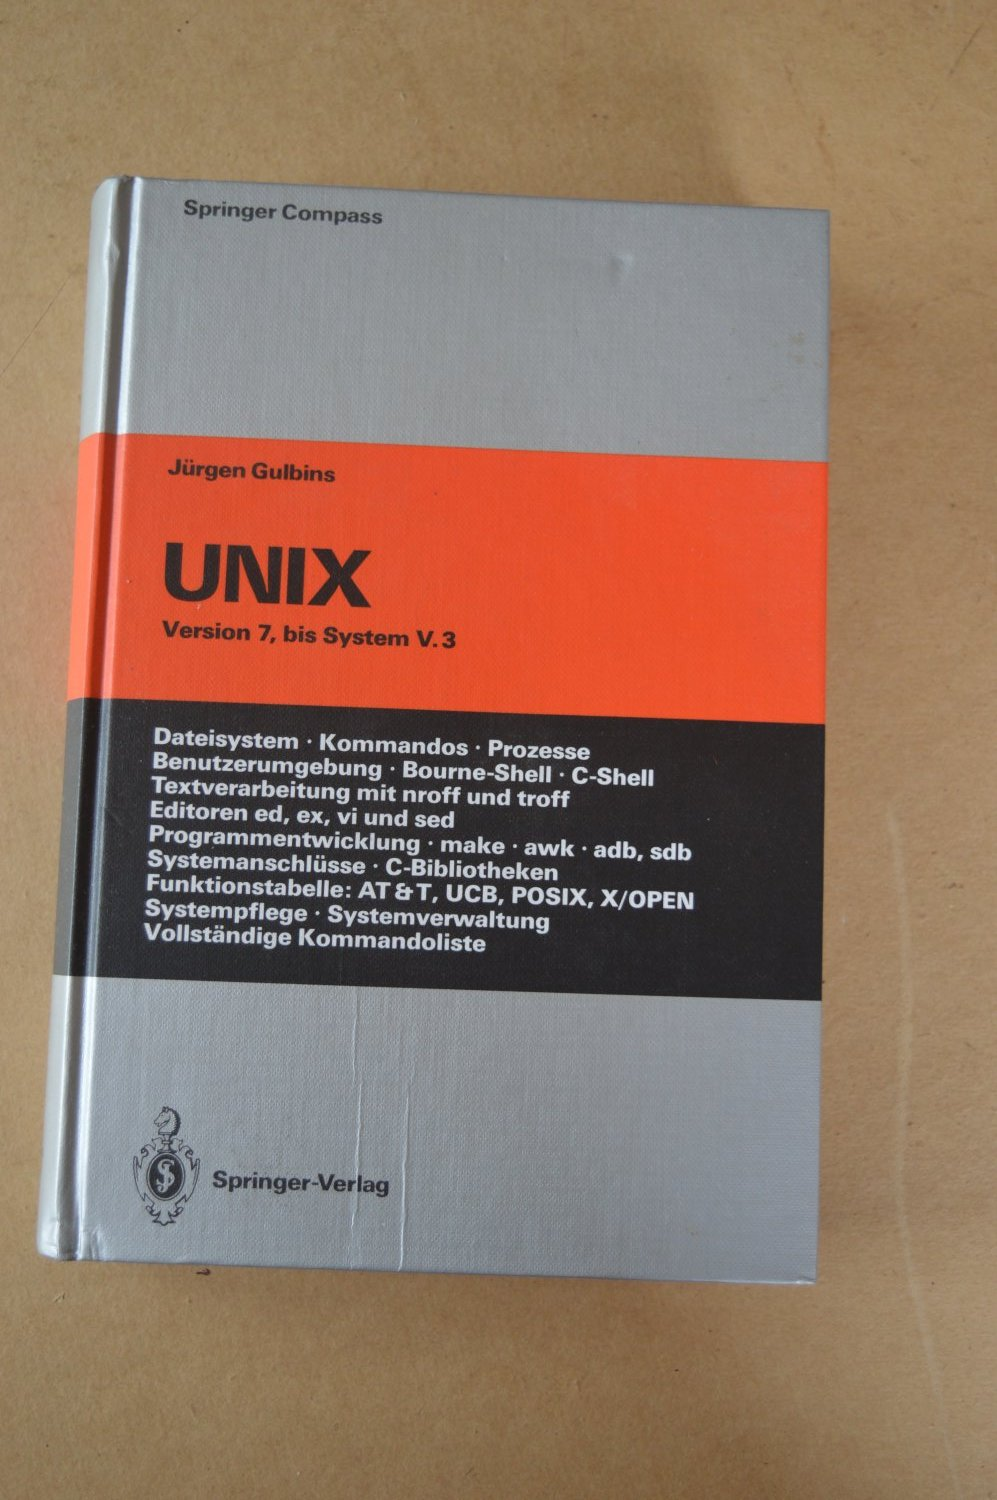
\includegraphics[height=0.95\textheight]{images/unix7}
    \end{center}
    \end{column}
    \end{columns}
\end{frame}

\point[demo]{Exploring \highlight{chroot}}

\begin{frame}[fragile]{Exploring \highlight{chroot}}
    \begin{code}[numbers=none]{}
> mkdir ./jail
> cd jail
> chroot . /bin/ls
chroot: failed to run command '/bin/ls': No such file or directory
> mkdir bin
> cp /bin/ls bin
> chroot . /bin/ls
chroot: failed to run command '/bin/ls': No such file or directory
    \end{code}
\end{frame}
\note[itemize]{
    \item First chroot -- Doesn't exist from our new root.
    \item Second chroot -- Exists but it can't find files on which ls depends.
}

\begin{frame}[fragile]{Exploring \highlight{chroot}}
    \vspace{-0.5em}
    \begin{code}[numbers=none]{}
> ldd /bin/ls
    libselinux.so.1 => /lib/x86_64-linux-gnu/libselinux.so.1 (0x00007f0097135000)
    libc.so.6 => /lib/x86_64-linux-gnu/libc.so.6 (0x00007f0096f0d000)
    libpcre2-8.so.0 => /lib/x86_64-linux-gnu/libpcre2-8.so.0 (0x00007f0096e76000)
    /lib64/ld-linux-x86-64.so.2 (0x00007f0097189000)
> cp --parents /lib/x86_64-linux-gnu/libselinux.so.1 /lib/x86_64-linux-gnu/libc.so.6 /lib/x86_64-linux-gnu/libpcre2-8.so.0 /lib64/ld-linux-x86-64.so.2 .
> ls
bin  lib  lib64
> ls lib/x86_64-linux-gnu/
libc.so.6  libpcre2-8.so.0  libselinux.so.1
    \end{code}
\end{frame}

\begin{frame}[fragile]{Exploring \highlight{chroot}}
    \begin{code}[numbers=none]{}
> chroot . /bin/ls
bin  lib  lib64
> chroot . /bin/ls /
bin  lib  lib64
> chroot . /bin/ls ..
bin  lib  lib64
> chroot . /bin/ls /bin
ls
    \end{code}
\end{frame}
\note[itemize]{
    \item ldd -- Lists dependencies
    \item cp -- Copy dependencies
    \item ls -- Show that these are now within our directory.
}

\begin{frame}[fragile]{Chroot Limitations}
    {\LARGE
    \begin{itemize}
        \item \highlight{Only filesystem isolation}
        \begin{itemize}
            \Large \item processes, network, etc. still accessible
        \end{itemize}
        \item Not very \highlight{user friendly}
        \item Not very \highlight{portable}
        \item \highlight{Jailbreak} is possible
    \end{itemize}
    }
\end{frame}
\note[itemize]{
    \item Can now run chroot . /bin/ls -- Everything is available from new root.
    \item Second chroot -- Shows that it considers our directory to be the root.
    \item Third chroot -- Shows we can't go to a parent directory.
}


\begin{frame}{1992}
    \begin{columns}
    \begin{column}{0.8\textwidth}
    \begin{center}
    \href{https://www.bell-labs.com/institute/blog/plan-9-bell-labs-cyberspace/}{
    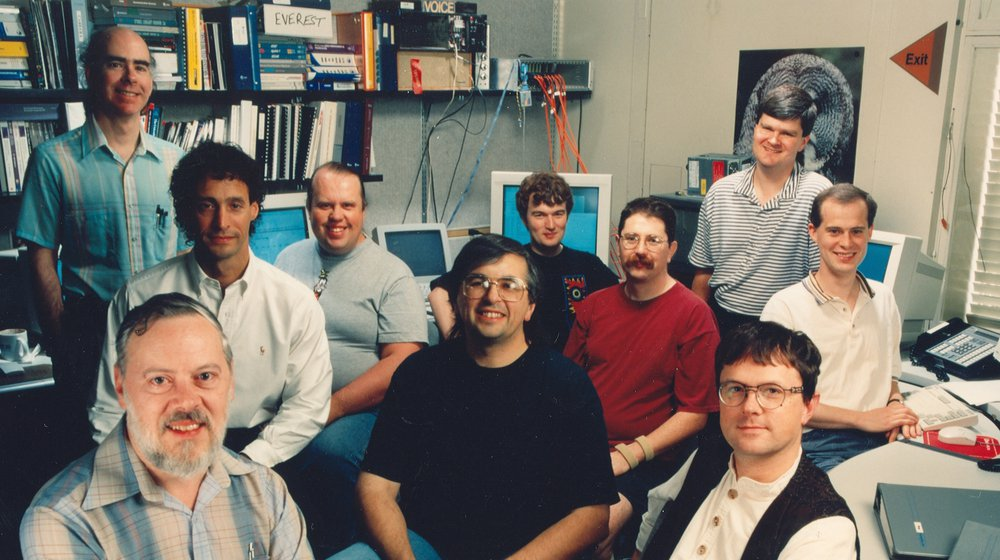
\includegraphics[width=\textwidth]{images/plan9}
}
\note[itemize]{
    \item Image shows members of the Bell Labs Computing Techniques Research Department, which developed Plan 9:
    \item (foreground, from left) Dennis Ritchie, Dave Presotto, Rob Pike,
    \item (background, from left) Tom Killian, Allen Eisdorfer, Tom Duff, Phil Winterbottom, Jim McKie, Howard Trickey and Sean Dorward.
}
    \end{center}
    \end{column}
     \begin{column}{0.25\textwidth}
    {\color{primary}\Large Plan 9}
    \vspace{1em}

    \large Introducing... \highlight{layered filesystem}
    \end{column}

    \end{columns}

\end{frame}

\point[Layered filesystem]{
    \begin{itemize}
        \item Projection on \highlight{read}
        \item Copy on \highlight{write}
    \end{itemize}
}

\begin{frame}[fragile]{Projection on \highlight{read}}
    \begin{center}
    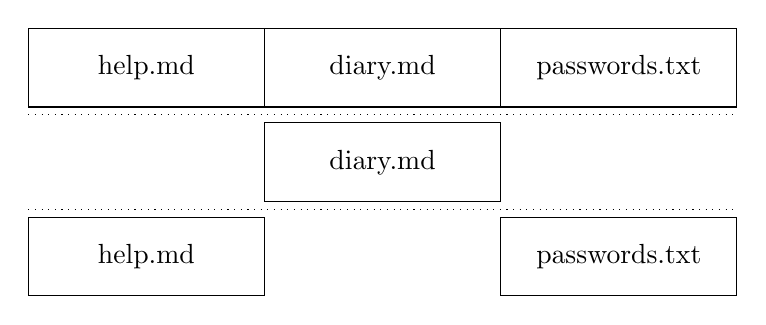
\begin{tikzpicture}[every fit/.style={inner sep=0pt, outer sep=0pt, draw}]

    \node [fit={(6,0) (9,1)}, label=center:{passwords.txt}] {};

    \node [fit={(3,1.2) (6,2.2)}, label=center:{diary.md}] {};
    \node [fit={(0,0) (3,1)}, label=center:{help.md}] {};

    \draw [dotted] (0,1.1) -- (9,1.1);

    \draw [dotted] (0,2.3) -- (9,2.3);

    \node [fit={(6,2.4) (9,3.4)}, label=center:{passwords.txt}] {};
    \node [fit={(3,2.4) (6,3.4)}, label=center:{diary.md}] {};
    \node [fit={(0,2.4) (3,3.4)}, label=center:{help.md}] {};
   \end{tikzpicture}
    \end{center}

\begin{code}[numbers=none]{}
> ls
passwords.txt help.md diary.md
\end{code}
\end{frame}
\note[itemize]{
    \item Two layers, and a projection giving us the perspective of a single merged layer.
    \item Lower layer is \textbf{\textit{read}} only.
}
\note{
    
}

\begin{frame}[fragile]{Copy on \highlight{write}}
\begin{code}[numbers=none]{}
> echo "1234" >> passwords.txt
\end{code}

    \begin{center}
    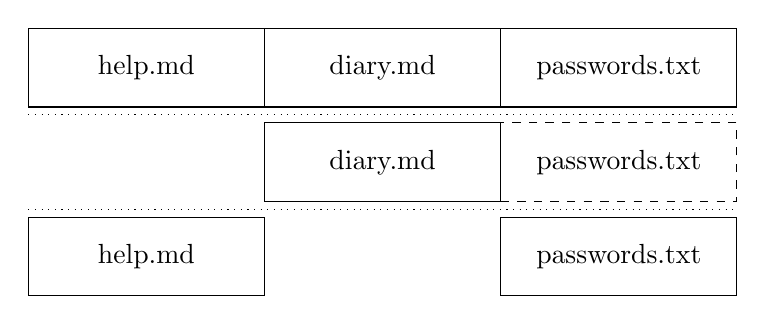
\begin{tikzpicture}[every fit/.style={inner sep=0pt, outer sep=0pt, draw}]

    \node [fit={(6,0) (9,1)}, label=center:{passwords.txt}] {};

    \node [fit={(3,1.2) (6,2.2)}, label=center:{diary.md}] {};
    \node [fit={(0,0) (3,1)}, label=center:{help.md}] {};

    \draw [dotted] (0,1.1) -- (9,1.1);

    \draw [dotted] (0,2.3) -- (9,2.3);

    \node [fit={(6,2.4) (9,3.4)}, label=center:{passwords.txt}] {};
    \node [fit={(3,2.4) (6,3.4)}, label=center:{diary.md}] {};
    \node [fit={(0,2.4) (3,3.4)}, label=center:{help.md}] {};

    \node [fit={(6,1.2) (9,2.2)}, dashed, label=center:{passwords.txt}] {};
   \end{tikzpicture}
    \end{center}
\end{frame}
\note[itemize]{
    \item Two layers:
    \item ~~Write to `passwords.txt' in the upper layer.
    \item ~~Leave `passwords.txt' in the lower layer unchanged.
}

\point[demo]{Exploring a \highlight{layered filesystem}}

\begin{frame}[fragile]{Exploring a \highlight{layered filesystem}}
    \begin{code}[numbers=none]{}
> mkdir lower upper worker merged
> echo "password1234" >> lower/passwords.txt
> touch lower/help.md upper/diary.md
> mount -t overlay -o lowerdir=lower,upperdir=upper,workdir=worker none merged
    \end{code}
\end{frame}

\begin{frame}[fragile]{Exploring a \highlight{layered filesystem}}
    \vspace{-0.5em}
    \begin{code}[numbers=none]{}
> ls merged
diary.md  help.md  passwords.txt
> ls upper
diary.md
> ls lower
> cat lower/passwords.txt
password1234
> echo "1234" >> merged/passwords.txt
> cat merged/passwords.txt
password1234
1234
> ls upper
diary.md passwords.txt
> cat lower/passwords.txt
password1234
    \end{code}
\end{frame}

\begin{frame}{2002}
    \begin{columns}
    \begin{column}{0.3\textwidth}
    {\color{primary}\Large Linux kernel 2.4.19}
    \vspace{1em}

    \large Introducing... \highlight{namespaces}
    \end{column}
    \begin{column}{0.7\textwidth}
    \begin{center}
    
\includegraphics[height=0.8\textheight]{images/linux-kernel}
    \end{center}
    \end{column}
    \end{columns}

\end{frame}

\begin{frame}{Linux Namespaces}
    {\LARGE
    \begin{description}
        \item[2002] \highlight{Mount} namespace
        \item[2006] \highlight{Unix Time-Sharing} namespace
        \item[2006] \highlight{Inter-process Communication} namespace
        \item[2008] \highlight{Process ID} namespace
        \item[2009] \highlight{Network} namespace
        \item[2013] \highlight{User} namespace
        \item[2016] \highlight{Control group} namespace
    \end{description}
    }
\end{frame}

\begin{frame}{2008}
    \begin{columns}
    \begin{column}{0.4\textwidth}
    {\color{primary} \Large LinuX Containers (LXC)}

    \end{column}
    \begin{column}{0.6\textwidth}
        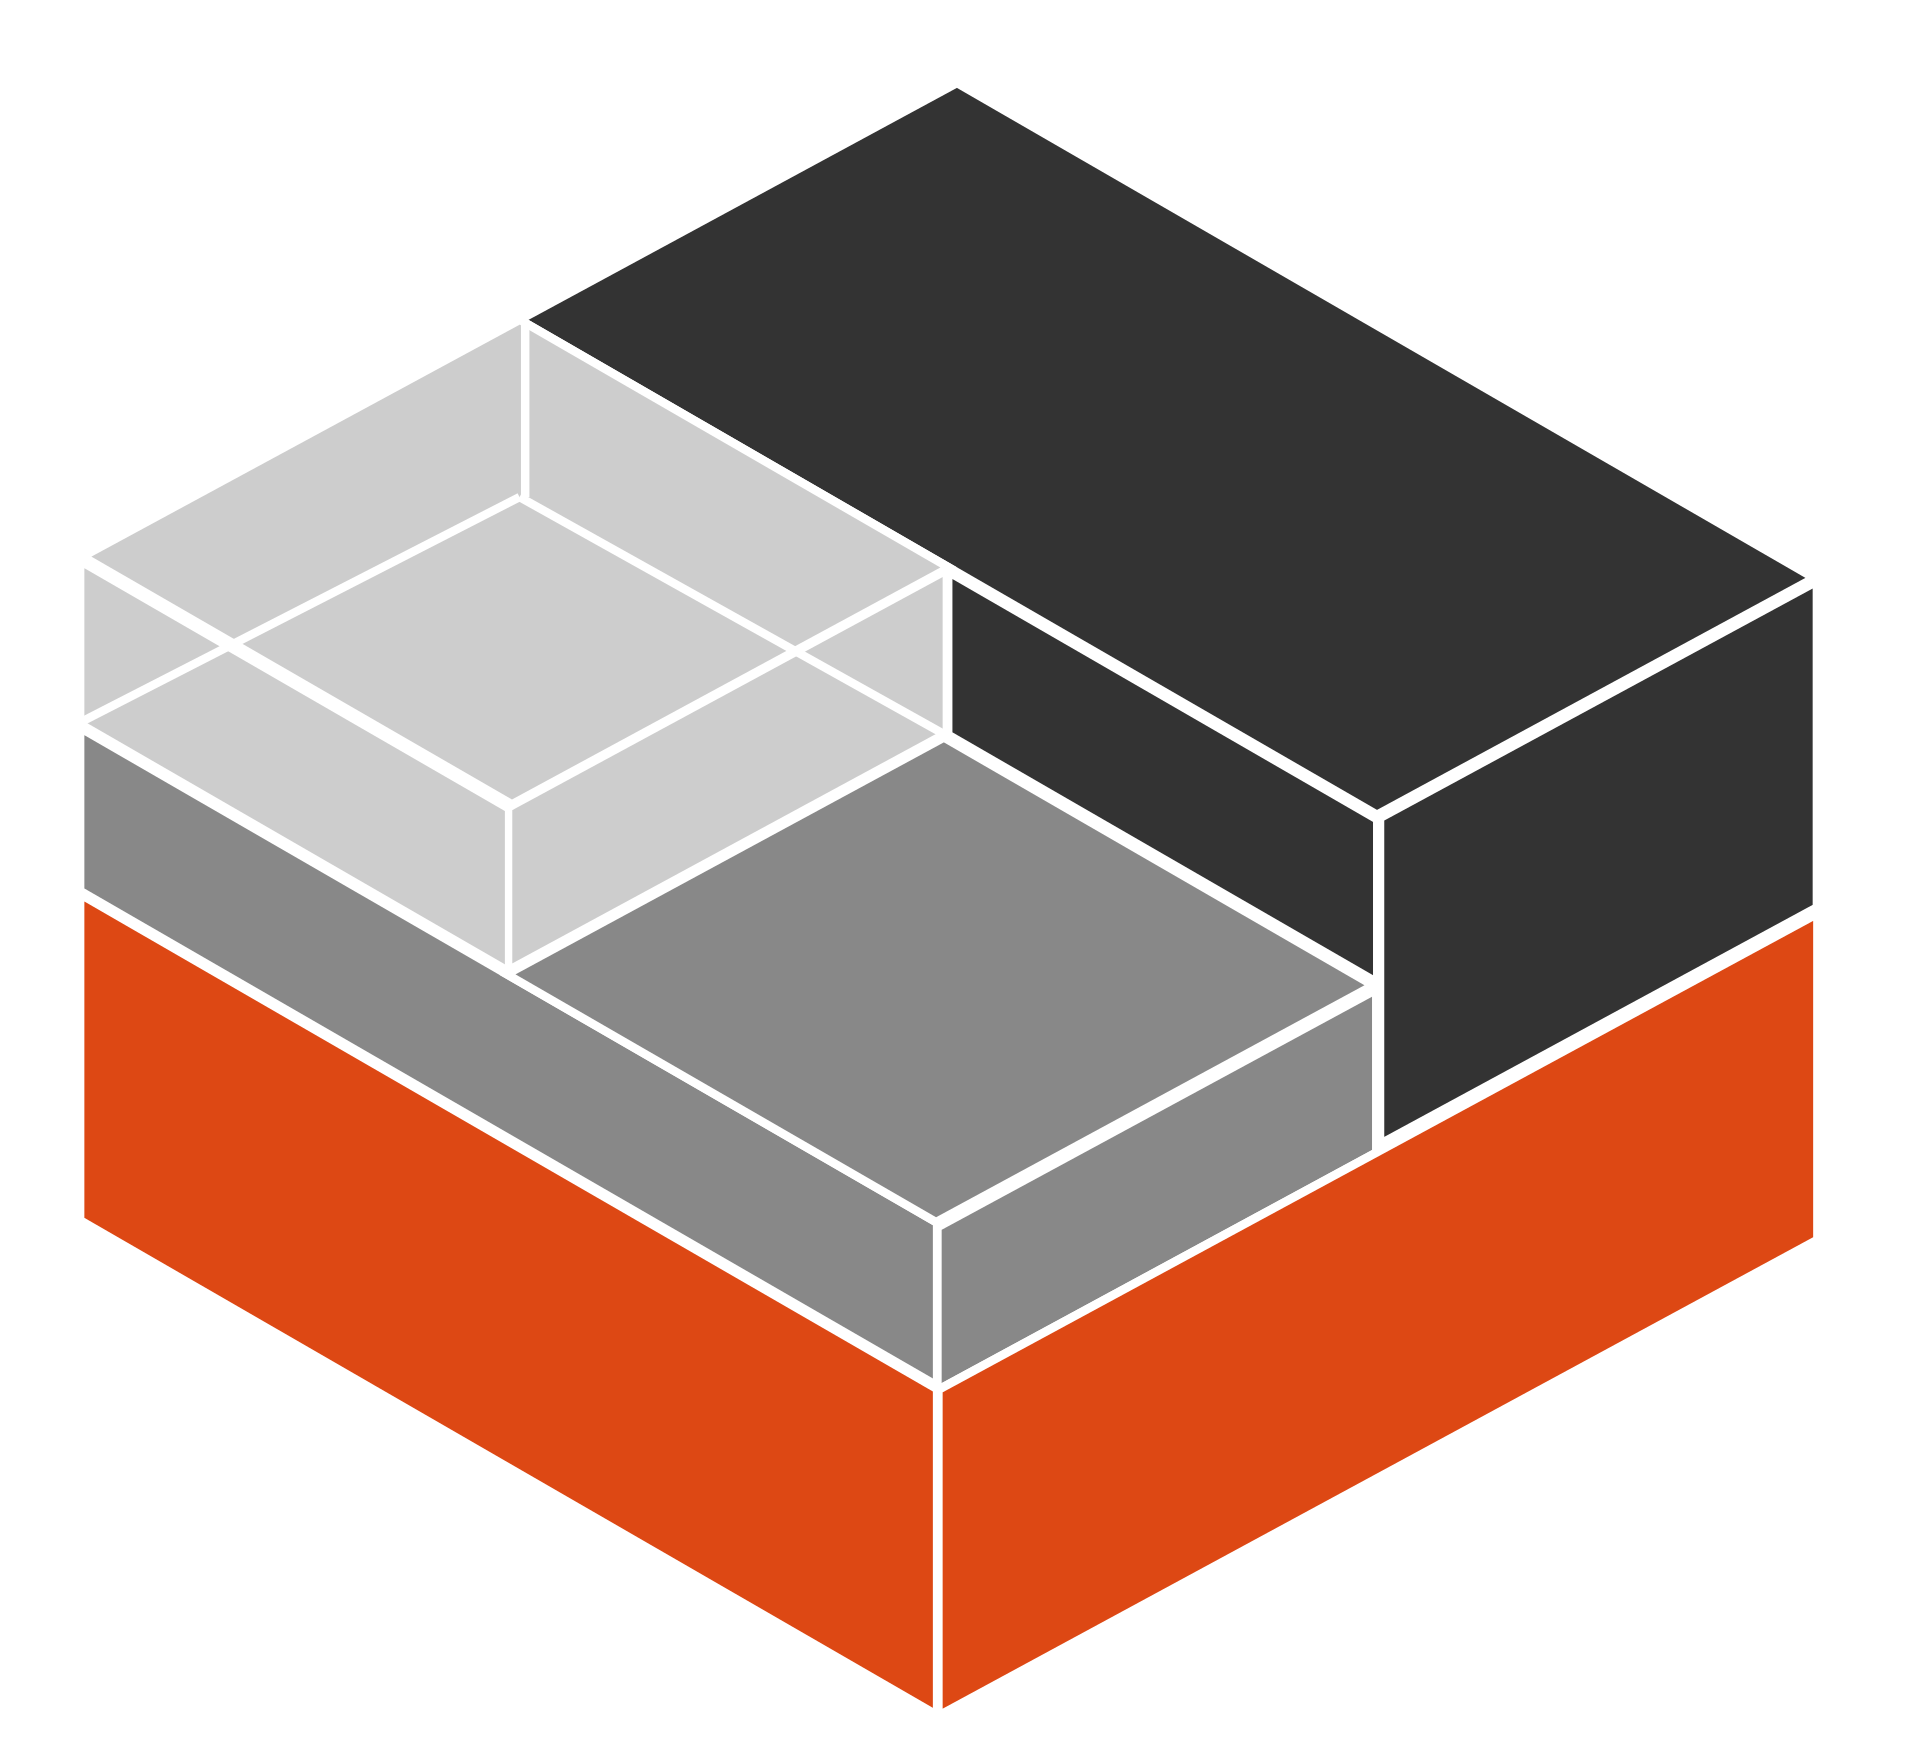
\includegraphics[width=\textwidth]{images/lxc}
    \end{column}
    \end{columns}
\end{frame}
\note{First to utilize namespaces, didn't require Linux patches}

\begin{frame}{2013}
    \begin{columns}
    \begin{column}{0.8\textwidth}
    \begin{center}
    \href{https://youtu.be/wW9CAH9nSLs}{
    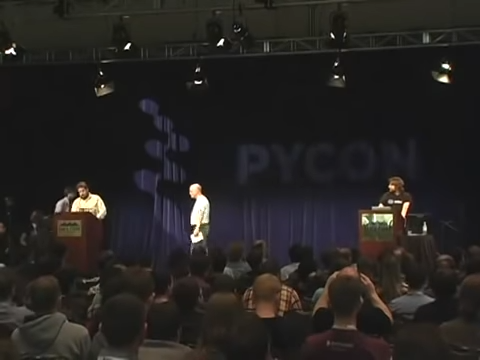
\includegraphics[height=0.8\textheight]{images/docker-release}
}
    \end{center}
    \end{column}
     \begin{column}{0.25\textwidth}
    {\color{primary}\Large PyCon 2013}
    \vspace{1em}

    \large Introducing... \highlight{Docker}
    \end{column}

    \end{columns}

\end{frame}

\quote[Nigel Poulton]{
    \highlight{Docker} was the magic that made Linux containers usable for mere mortals.
}


\section{The Language of Containers}

\definition{Container}{
    A \highlight{running process} created from a container image.
    Typically isolated from the host system.
}

\definition{Container Image}{
    A set of files that can be used to \highlight{create a container}.
}
\note{
    The mount point for starting containers.\\
    In Docker and rkt the image is just a collection of layers.\\
    i.e. lower, and upper, repeatedly stacked on top of themselves.\\
    In LXC it is just one layer.
}

\begin{frame}[fragile]{Container Image}
    \begin{columns}
    \begin{column}{0.4\textwidth}
    \begin{center}
    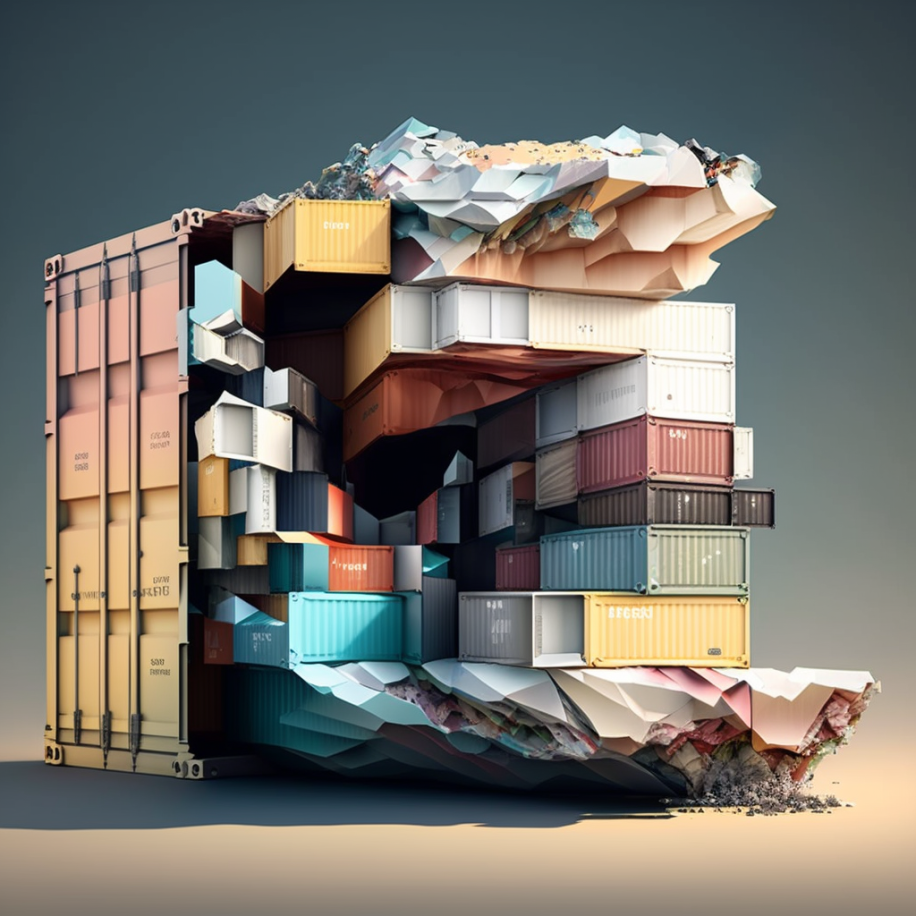
\includegraphics[height=0.8\textheight]{images/container-image}

    \end{center}
    \end{column}
    \begin{column}{0.6\textwidth}
    \begin{code}[numbers=none]{}
> docker run -it ubuntu /bin/bash
root@f2b0b0c0b0b0:/# ls
bin   dev  home  lib64  mnt  proc  run   srv
root@f2b0b0c0b0b0:/# exit
    \end{code}
    \begin{code}[numbers=none]{}
> docker run -it ubuntu /bin/ls
bin   dev  home  lib64  mnt  proc  run   srv
    \end{code}
    \end{column}
    \end{columns}
\end{frame}

\definition{Container Engine}{
    A tool to \highlight{create} and \highlight{manage} containers.
    Often also manages container images.
}

\point[Container Engines]{
    \begin{itemize}
        \item Docker
        \item rkt
        \item LXC
        \item runC
        \item Containerd
        \item CRI-O
        \item Podman
    \end{itemize}
}

\point[Creating a container image]{
    \vspace{3mm}
    To create a container image,
    we need to \highlight{create a collection of image layers}.

    \vspace{3mm}
    Fortunately, this is no longer a manual process...
    \pause
    
    \vspace{3mm}
    Instead we use a \highlight{build file}, or image blueprints.
}

\definition{Build File}{
    File containing the \highlight{instructions} for \highlight{creating a container image}.
}

\begin{frame}[fragile]{Build File}
\begin{code}[language=docker]{Dockerfile}
FROM ubuntu
RUN apt-get update 
RUN apt-get install -y cowsay
CMD ["/usr/games/cowsay", "Hello World"]
\end{code}

\pause
\begin{code}[numbers=none]{}
> docker build -t cowsay .
\end{code}

\pause
\begin{code}[numbers=none]{}
> docker run cowsay
\end{code}
\end{frame}

\begin{frame}[fragile]
    \begin{columns}
    \hspace{1em}
    \begin{column}{0.6\textwidth}
    \begin{code}[language=docker]{Dockerfile}
FROM ubuntu
RUN apt-get update 
RUN apt-get install -y cowsay
CMD ["/usr/games/cowsay", "Hello World"]
    \end{code}
    \end{column}

    \begin{column}{0.4\textwidth}
    \begin{center}
    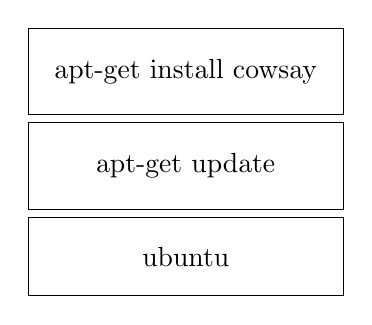
\begin{tikzpicture}[every fit/.style={inner sep=0pt, outer sep=0pt, draw}]
        \node [fit={(0,0) (4,1)}, label=center:{ubuntu}] {};
        \node [fit={(0,1.1) (4,2.2)}, label=center:{apt-get update}] {};
        \node [fit={(0,2.3) (4,3.4)}, label=center:{apt-get install cowsay}] {};

    \end{tikzpicture}
    \end{center}
    \end{column}
    \end{columns}
\end{frame}

\begin{frame}[fragile]
    \begin{columns}
    \hspace{1em}
    \begin{column}{0.6\textwidth}
    \begin{code}[language=docker]{Dockerfile}
FROM ubuntu
RUN apt-get update 
RUN apt-get install -y cowsay
RUN rm -rf /var/lib/apt/lists/*
CMD ["/usr/games/cowsay", "Hello World"]
    \end{code}
    \end{column}

    \begin{column}{0.4\textwidth}
    \begin{center}
    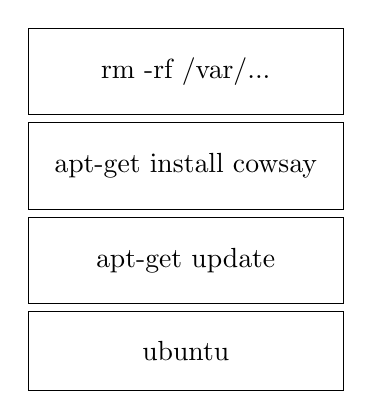
\begin{tikzpicture}[every fit/.style={inner sep=0pt, outer sep=0pt, draw}]
        \node [fit={(0,0) (4,1)}, label=center:{ubuntu}] {};
        \node [fit={(0,1.1) (4,2.2)}, label=center:{apt-get update}] {};
        \node [fit={(0,2.3) (4,3.4)}, label=center:{apt-get install cowsay}] {};
        \node [fit={(0,3.5) (4,4.6)}, label=center:{rm -rf /var/...}] {};

    \end{tikzpicture}
    \end{center}
    \end{column}
    \end{columns}
\end{frame}

\begin{frame}[fragile]
    \begin{columns}
    \hspace{1em}
    \begin{column}{0.6\textwidth}
    \begin{code}[language=docker]{Dockerfile}
FROM ubuntu
RUN apt-get update && \
    apt-get install -y cowsay && \
    rm -rf /var/lib/apt/lists/*
CMD ["/usr/games/cowsay", "Hello World"]
    \end{code}
    \end{column}

    \begin{column}{0.4\textwidth}
    \begin{center}
    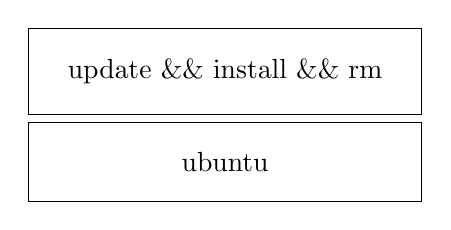
\begin{tikzpicture}[every fit/.style={inner sep=0pt, outer sep=0pt, draw}]
        \node [fit={(0,0) (5,1)}, label=center:{ubuntu}] {};
        \node [fit={(0,1.1) (5,2.2)}, label=center:{update \&\& install \&\& rm}] {};

    \end{tikzpicture}
    \end{center}
    \end{column}
    \end{columns}
\end{frame}

\questionanswer{Where did \highlight{ubuntu} come from?}{
    Our final definition --- a \highlight{container registry}.
}

\definition{Container Registry}{
    A file sharing platform that \highlight{hosts container images}.
    Container images are \highlight{pulled} (downloaded) from registries.
}


\section{Virtual Machines}

\begin{frame}
    \begin{columns}
        \hspace{-4.5em}
        \begin{column}{0.4\textwidth}
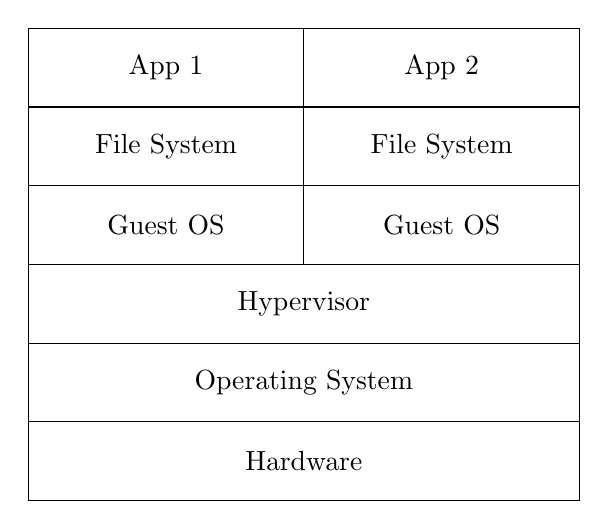
\begin{tikzpicture}[every fit/.style={inner sep=0pt, outer sep=0pt, draw}]
    \begin{scope}[y=1cm]
        \node [fit={(0,0) (7,1)}, label=center:{Hardware}] {};
    \end{scope}

    \begin{scope}[yshift=1cm,y=1cm]
        \node [fit={(0,0) (7,1)}, label=center:{Operating System}] {};
    \end{scope}

    \begin{scope}[yshift=2cm,y=1cm]
        \node [fit={(0,0) (7,1)}, label=center:{Hypervisor}] {};
    \end{scope}

    \begin{scope}[yshift=3cm,y=1cm]
        \node [fit={(0,0) (3.5,1)}, label=center:{Guest OS}] {};
        \node [fit={(3.5,0) (7,1)}, label=center:{Guest OS}] {};
    \end{scope}

    \begin{scope}[yshift=4cm,y=1cm]
        \node [fit={(0,0) (3.5,1)}, label=center:{File System}] {};
        \node [fit={(3.5,0) (7,1)}, label=center:{File System}] {};
    \end{scope}

    \begin{scope}[yshift=5cm,y=1cm]
        \node [fit={(0,0) (3.5,1)}, label=center:{App 1}] {};
        \node [fit={(3.5,0) (7,1)}, label=center:{App 2}] {};
    \end{scope}

\end{tikzpicture}
\end{column}
\pause
\begin{column}{0.45\textwidth}
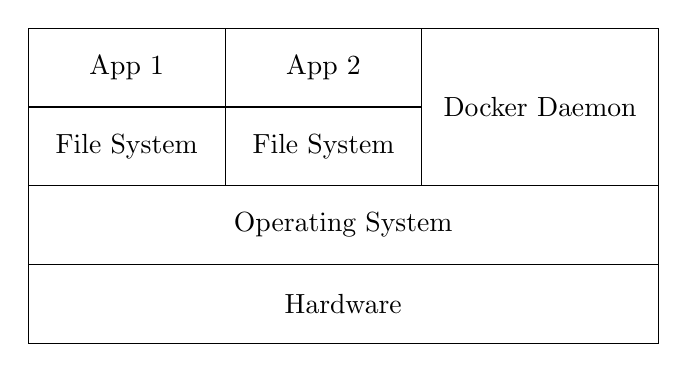
\begin{tikzpicture}[every fit/.style={inner sep=0pt, outer sep=0pt, draw}]
    \begin{scope}[y=1cm]
    \node [fit={(0,0) (8,1)}, label=center:{Hardware}] {};
    \end{scope}

    \begin{scope}[yshift=1cm,y=1cm]
        \node [fit={(0,0) (8,1)}, label=center:{Operating System}] {};
    \end{scope}

    \begin{scope}[yshift=2cm,y=2cm]
    \node [fit={(0,0) (2.5,0.5)}, label=center:{File System}] {};
    \node [fit={(0,0.5) (2.5,1)}, label=center:{App 1}] {};
    \node [fit={(2.5,0) (5,0.5)}, label=center:{File System}] {};
    \node [fit={(2.5,0.5) (5,1)}, label=center:{App 2}] {};
    \node [fit={(5,0) (8,1)}, label=center:{Docker Daemon}] {};
    \end{scope}
\end{tikzpicture}
\end{column}
\end{columns}
\end{frame}

\point[Isolation]{
    Virtual machines are used for \highlight{machine isolation}.
    \vspace{1em}

    Containers are used for \highlight{process isolation}.
}

\begin{frame}{Size Comparison}

    I want \highlight{10} flask servers running on Ubuntu 22.

    \normalsize
    \begin{align*}
        \text{Ubuntu 22} &\simeq 3.8GB \\
        \text{Python 3.6} &\simeq 232MB \\
        \text{Flask} &\simeq 11.1MB \\
        \text{My App} &\simeq 12K 
    \end{align*}

\begin{columns}
    \begin{column}{0.5\textwidth}
    {\color{primary} Virtual Machine}
    \begin{align*}
        \text{Image Size} &= 3.8GB + 232MB \\
                          &+ 11.1MB + 12K\\
        &= 4.04GB \\
        \text{Total Space} &= 4.04GB * 10 \\
        &= 40.4GB
    \end{align*}
    \end{column}
    \begin{column}{0.5\textwidth}
    {\color{primary} Container}
    \begin{align*}
        \text{Image Size} &= 12K \\
        \text{Layer Size} &= 3.8GB + 232MB + 11.1MB \\
                             &= 4.04GB \\
        \text{Total Space} &= (12K * 10) + 4.04GB \\
                           &\simeq 4.04GB
    \end{align*}
    \end{column}
\end{columns}
\end{frame}

\questionanswer{When would I want a \highlight{virtual machine}?}{
    \begin{itemize}
        \item Running a \highlight{different operating system}.
        \item \highlight{Unique hardware requirements} such as emulating old computer hardware.
        \item Where \highlight{security} is crucial virtual machines can offer greater isolation.
    \end{itemize}
}

\questionanswer{When would I want a \highlight{container}?}{
    \begin{itemize}
        \item Running a \highlight{single application}.
        \item \highlight{Lightweight} and \highlight{fast} to startup.
        \item Running \highlight{many containers} on the same system.
    \end{itemize}
}

\point[Combined Use Cases]{
%    \Large
    Often virtual machines and containers are \highlight{combined}.

    \vspace{1em}
    e.g. If you deploy containers on Google Kubernetes Engine, the containers run inside of virtual machines on Google's hardware.
}


\section{Use Cases}

\point[Dependency Management]{
Containers provide a reliable,
if brute force,
way to \highlight{manage dependencies}.

\vspace{4mm}
Wrap the whole machine state up and ship it.
}

\point[Continuous Integration]{
Containers allow developers to locally
\highlight{replicate the same test environment}
as the CI system.
}

\point[Continuous Delivery]{
Containers allow teams to package, deploy, and manage applications more efficiently.

\vspace{4mm}
Containers can be used to \highlight{deploy} on cloud platforms or on-premise servers with \highlight{minimal manual configuration}.
}

\point[Scaling]{
Containers allow applications to be \highlight{scaled up or down quickly and efficiently}.
}

\point[Microservices]{
Containers make it easy to deploy and manage \highlight{individual services independently}.
}

\point[Serverless]{
Containers are the basis for \highlight{serverless computing}.
}


\section{Docker}

\image{images/dock-workers}

\command{docker build [context]}{
    Run each instruction in the \highlight{blueprint (Dockerfile)}
    to \highlight{build} each layer resulting in the top-level layer (\highlight{image}).
}{
    \item[-f] The Dockerfile to use (default: [context]/Dockerfile)
\item[-t] The tag (name) of the image to build
}

\command{docker run [image]}{
    Run a \highlight{container} from the specified \highlight{image}.
}{
    \item[-d] Run the container in the background
\item[-p] Publish a container's port to the host
\item[-v] Mount a volume
\item[-e] Set environment variables
\item[-i] Keep STDIN open even if not attached
\item[-t] Allocate a pseudo-TTY
}

\command{docker exec [container]}{
    Run a command in a \highlight{running container}.
}{
    \item[-d] Run the command in the background
\item[-e] Set environment variables
\item[-i] Keep STDIN open even if not attached
\item[-t] Allocate a pseudo-TTY
}

\command{docker ps}{
    List running containers.
}{
    \item[-a] Show all containers (default shows just running)
\item[-f] Filter output based on conditions provided
}

\command{docker stop [container]}{
    Stop a running container.
}{
    \item[-t] Seconds to wait for stop before killing it
}

\command{docker rm [container]}{
    Remove a container.
}{
    \item[-f] Force the removal of a running container (uses SIGKILL)
\item[-v] Remove the volumes associated with the container
}

\command{docker images}{
    List images.
}{
    \item[-a] Show all images (default hides intermediate images)
    \item[-f] Filter output based on conditions provided
}

\command{docker rmi [image]}{
    Remove an image.
}{
    \item[-f] Force removal of the image
}

\commandnoarg{docker pull [image]}{
    Pull an image or a repository from a registry.
}

\commandnoarg{docker push [image]}{
    Push an image or a repository to a registry.
}

\section{Examples}

\begin{frame}[fragile]{Structurizr}
    \begin{code}[numbers=none]{}
> git clone git@github.com:CSSE6400/software-architecture.git
> cd software-architecture/slides/microkernel/c4_model
> docker run -it --rm -p 8080:8080 -v $(pwd):/usr/local/structurizr structurizr/lite
    \end{code}

Open in browser: \url{http://localhost:8080}
\end{frame}

\begin{frame}[fragile]{GitLab}
    \begin{code}[numbers=none]{}
> mkdir gitlab
> export GITLAB_HOME=$(pwd)/gitlab
> docker run -it --rm -d -p 223:80 --shm-size 256m -v ${GITLAB_HOME}/config:/etc/gitlab -v ${GITLAB_HOME}/logs:/var/logs/gitlab -v ${GITLAB_HOME}/data:/var/opt/gitlab gitlab/gitlab-ee:latest
> cat ./gitlab/config/initial_password
    \end{code}

Open in browser: \url{http://localhost:223}
\end{frame}

\begin{frame}[fragile]{Doom}
    \begin{code}[numbers=none]{}
> docker run -it --rm -p 224:6901 -e VNC_PW=password kasmweb/doom:1.12.0
    \end{code}

Open in browser: \url{http://localhost:224}

Username: kasm\_user

Password: password
\end{frame}



\section{Docker Compose}

\point[Exercise]{
    We want to create \highlight{multiple} containers that \highlight{work together}.
    \pause

    \vspace{4mm}
    But we don't want to remember all the \highlight{commands to start and manage} the containers and get them to talk to each other\dots
}

\point[When faced with tedium]{
    Script it!
}

\begin{frame}[fragile]
    \begin{code}[language=bash]{start.sh}
docker build -t frontend ./frontend
docker build -t backend ./backend

docker run -p 3000:3000 -v ./frontend:/app -e ... -d frontend
docker run -p 8081:8081 -v ./backend:/app -e ... -d backend
docker run -p 80:80 -v ./nginx.conf:/etc/nginx/nginx.conf -d nginx
    \end{code}
\end{frame}

\point{This turns out to be very common\dots

\pause
\vspace{4mm}
Introducing\dots \highlight{Docker Compose}
}

\definecolor{Aquamarine}{HTML}{00B5BE}
\definecolor{Peach}{HTML}{F7965A}
\definecolor{CarnationPink}{HTML}{F282B4}
\definecolor{LimeGreen}{HTML}{8DC73E}

\begin{frame}[fragile]
    \begin{columns}
    \begin{column}{0.4\textwidth}
    \vspace{-20em}
    \begin{code}[language=bash,escapechar=!]{start.sh}
docker build
    -t frontend
    !\colorbox{Aquamarine}{./frontend}!

docker run
    !\colorbox{Peach}{-p 3000:3000}!
    !\colorbox{CarnationPink}{-v ./frontend:/app}!
    !\colorbox{LimeGreen}{-e ...}!
    -d 
    frontend
    \end{code}
    \end{column}%
    \begin{column}{0.5\textwidth}
    \begin{code}[numbers=none,escapechar=!]{docker-compose.yml}
version: '3'
services:
  frontend:
    !\colorbox{Aquamarine}{build: ./frontend}!
    ports:
      !\colorbox{Peach}{- "3000:3000"}!
    volumes:
      !\colorbox{CarnationPink}{- ./frontend:/app}!
    environment:
      !\colorbox{LimeGreen}{- ...}!
  backend:
    build: ./backend
    ports:
      - "8081:8081"
    volumes:
      - ./backend:/app
    environment:
      - ...
  nginx:
    image: nginx
    ports:
      - "80:80"
    volumes:
      - ./nginx.conf:/etc/nginx/nginx.conf
    depends_on:
      - frontend
      - backend
    \end{code}
    \end{column}
    \end{columns}
\end{frame}

\command{docker-compose up}{
    Create and run containers.
}{
    \item[-d] Detached mode: Run containers in the background, print new container names.
    \item[--build] Rebuild containers if necessary.
}

\command{docker-compose down}{
    Stop and remove containers, networks, images, and volumes.
}{
    \item[-v] Remove named volumes declared in the `volumes' section of the Compose file and anonymous volumes attached to containers.
\item[-t] Specify a shutdown timeout in seconds.
}

\commandnoarg{docker-compose ps}{
    List containers.
}

\command{docker-compose logs}{
    View output from containers.
}{
    \item[-f] Follow log output.
}

\command{docker-compose exec [service]}{
    Run a command in a running container.
}{
    \item[-d] Detached mode: Run command in the background.
\item[-T] Disable pseudo-tty allocation. By default `docker-compose exec' allocates a TTY.
\item[-e] Set environment variables.
}

\command{docker-compose build}{
    Build or rebuild services.
}{
    \item[--no-cache] Do not use cache when building the image.
\item[--pull] Always attempt to pull a newer version of the image.
    
}

\begin{frame}{In the practical this week...}
    \centering
    
\includegraphics[width=.95\textwidth]{images/practical}
\end{frame}


\begin{frame}
    \centering
\href{https://xkcd.com/1988/}{
    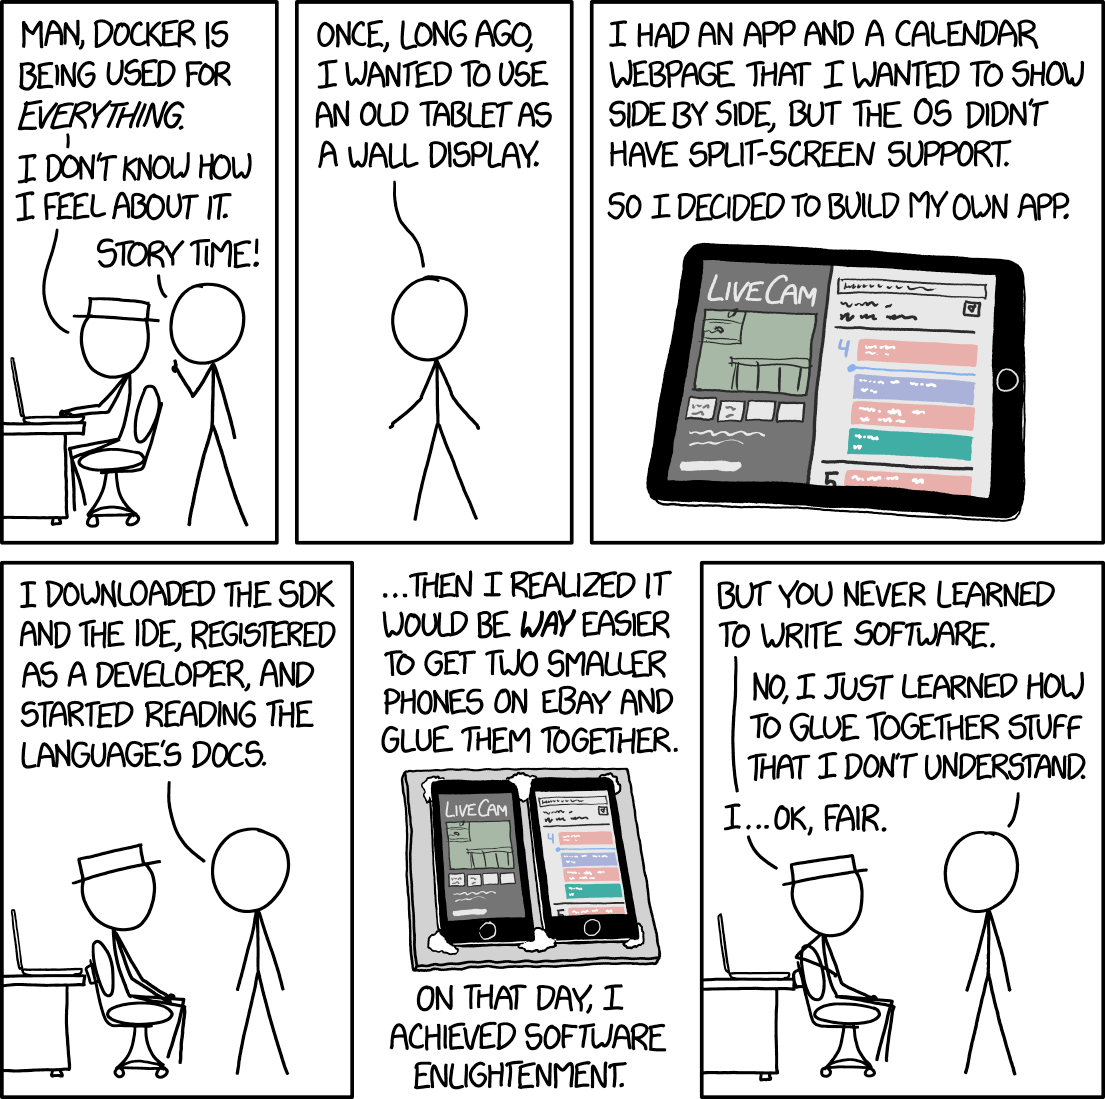
\includegraphics[height=0.9\textheight]{./images/xkcd1988}
}

\url{https://xkcd.com/1988/}
\end{frame}


% \references{articles,books}

\end{document}
